\documentclass{extbook}[14pt]
\usepackage{multicol, enumerate, enumitem, hyperref, color, soul, setspace, parskip, fancyhdr, amssymb, amsthm, amsmath, bbm, latexsym, units, mathtools}
\everymath{\displaystyle}
\usepackage[headsep=0.5cm,headheight=0cm, left=1 in,right= 1 in,top= 1 in,bottom= 1 in]{geometry}
\usepackage{dashrule}  % Package to use the command below to create lines between items
\newcommand{\litem}[1]{\item #1

\rule{\textwidth}{0.4pt}}
\pagestyle{fancy}
\lhead{}
\chead{Answer Key for Makeup Progress Quiz 3 Version A}
\rhead{}
\lfoot{4315-3397}
\cfoot{}
\rfoot{Fall 2020}
\begin{document}
\textbf{This key should allow you to understand why you choose the option you did (beyond just getting a question right or wrong). \href{https://xronos.clas.ufl.edu/mac1105spring2020/courseDescriptionAndMisc/Exams/LearningFromResults}{More instructions on how to use this key can be found here}.}

\textbf{If you have a suggestion to make the keys better, \href{https://forms.gle/CZkbZmPbC9XALEE88}{please fill out the short survey here}.}

\textit{Note: This key is auto-generated and may contain issues and/or errors. The keys are reviewed after each exam to ensure grading is done accurately. If there are issues (like duplicate options), they are noted in the offline gradebook. The keys are a work-in-progress to give students as many resources to improve as possible.}

\rule{\textwidth}{0.4pt}

\begin{enumerate}\litem{
Construct the lowest-degree polynomial given the zeros below. Then, choose the intervals that contain the coefficients of the polynomial in the form $ax^3+bx^2+cx+d$.
\[ \frac{-4}{5}, 2, \text{ and } \frac{7}{5} \]

The solution is \( 25x^{3} -65 x^{2} +2 x + 56 \), which is option C.\begin{enumerate}[label=\Alph*.]
\item \( a \in [24, 31], b \in [-72, -62], c \in [1, 7], \text{ and } d \in [-56, -55] \)

$25x^{3} -65 x^{2} +2 x -56$, which corresponds to multiplying everything correctly except the constant term.
\item \( a \in [24, 31], b \in [57, 69], c \in [1, 7], \text{ and } d \in [-56, -55] \)

$25x^{3} +65 x^{2} +2 x -56$, which corresponds to multiplying out $(5x -4)(x + 2)(5x + 7)$.
\item \( a \in [24, 31], b \in [-72, -62], c \in [1, 7], \text{ and } d \in [53, 61] \)

* $25x^{3} -65 x^{2} +2 x + 56$, which is the correct option.
\item \( a \in [24, 31], b \in [-105, -101], c \in [138, 141], \text{ and } d \in [-56, -55] \)

$25x^{3} -105 x^{2} +138 x -56$, which corresponds to multiplying out $(5x -4)(x -2)(5x -7)$.
\item \( a \in [24, 31], b \in [-11, -3], c \in [-87, -79], \text{ and } d \in [53, 61] \)

$25x^{3} -5 x^{2} -82 x + 56$, which corresponds to multiplying out $(5x -4)(x + 2)(5x -7)$.
\end{enumerate}

\textbf{General Comment:} To construct the lowest-degree polynomial, you want to multiply out $(5x + 4)(x -2)(5x -7)$
}
\litem{
Construct the lowest-degree polynomial given the zeros below. Then, choose the intervals that contain the coefficients of the polynomial in the form $x^3+bx^2+cx+d$.
\[ 2 + 4 i \text{ and } -4 \]

The solution is \( x^{3} +4 x + 80 \), which is option A.\begin{enumerate}[label=\Alph*.]
\item \( b \in [-1.82, 0.38], c \in [3.17, 4.11], \text{ and } d \in [79, 85] \)

* $x^{3} +4 x + 80$, which is the correct option.
\item \( b \in [-1.82, 0.38], c \in [3.17, 4.11], \text{ and } d \in [-80, -76] \)

$x^{3} +4 x -80$, which corresponds to multiplying out $(x-(2 + 4 i))(x-(2 - 4 i))(x -4)$.
\item \( b \in [0.07, 1.76], c \in [1.42, 3.02], \text{ and } d \in [-10, -5] \)

$x^{3} + x^{2} +2 x -8$, which corresponds to multiplying out $(x -2)(x + 4)$.
\item \( b \in [0.07, 1.76], c \in [-0.67, 0.1], \text{ and } d \in [-18, -10] \)

$x^{3} + x^{2} -16$, which corresponds to multiplying out $(x -4)(x + 4)$.
\item \( \text{None of the above.} \)

This corresponds to making an unanticipated error or not understanding how to use nonreal complex numbers to create the lowest-degree polynomial. If you chose this and are not sure what you did wrong, please contact the coordinator for help.
\end{enumerate}

\textbf{General Comment:} Remember that the conjugate of $a+bi$ is $a-bi$. Since these zeros always come in pairs, we need to multiply out $(x-(2 + 4 i))(x-(2 - 4 i))(x-(-4))$.
}
\litem{
Construct the lowest-degree polynomial given the zeros below. Then, choose the intervals that contain the coefficients of the polynomial in the form $x^3+bx^2+cx+d$.
\[ 3 + 4 i \text{ and } 2 \]

The solution is \( x^{3} -8 x^{2} +37 x -50 \), which is option B.\begin{enumerate}[label=\Alph*.]
\item \( b \in [0, 2], c \in [-6.65, -5.66], \text{ and } d \in [8, 12] \)

$x^{3} + x^{2} -6 x + 8$, which corresponds to multiplying out $(x -4)(x -2)$.
\item \( b \in [-14, -4], c \in [37, 37.08], \text{ and } d \in [-56, -49] \)

* $x^{3} -8 x^{2} +37 x -50$, which is the correct option.
\item \( b \in [6, 11], c \in [37, 37.08], \text{ and } d \in [47, 56] \)

$x^{3} +8 x^{2} +37 x + 50$, which corresponds to multiplying out $(x-(3 + 4 i))(x-(3 - 4 i))(x + 2)$.
\item \( b \in [0, 2], c \in [-5.69, -4.9], \text{ and } d \in [3, 7] \)

$x^{3} + x^{2} -5 x + 6$, which corresponds to multiplying out $(x -3)(x -2)$.
\item \( \text{None of the above.} \)

This corresponds to making an unanticipated error or not understanding how to use nonreal complex numbers to create the lowest-degree polynomial. If you chose this and are not sure what you did wrong, please contact the coordinator for help.
\end{enumerate}

\textbf{General Comment:} Remember that the conjugate of $a+bi$ is $a-bi$. Since these zeros always come in pairs, we need to multiply out $(x-(3 + 4 i))(x-(3 - 4 i))(x-(2))$.
}
\litem{
Construct the lowest-degree polynomial given the zeros below. Then, choose the intervals that contain the coefficients of the polynomial in the form $ax^3+bx^2+cx+d$.
\[ -6, \frac{-7}{4}, \text{ and } \frac{1}{4} \]

The solution is \( 16x^{3} +120 x^{2} +137 x -42 \), which is option A.\begin{enumerate}[label=\Alph*.]
\item \( a \in [11, 21], b \in [117, 121], c \in [134, 138], \text{ and } d \in [-47, -41] \)

* $16x^{3} +120 x^{2} +137 x -42$, which is the correct option.
\item \( a \in [11, 21], b \in [-122, -115], c \in [134, 138], \text{ and } d \in [42, 43] \)

$16x^{3} -120 x^{2} +137 x + 42$, which corresponds to multiplying out $(x -6)(4x -7)(4x + 1)$.
\item \( a \in [11, 21], b \in [-72, -70], c \in [-152, -143], \text{ and } d \in [42, 43] \)

$16x^{3} -72 x^{2} -151 x + 42$, which corresponds to multiplying out $(x -6)(4x + 7)(4x -1)$.
\item \( a \in [11, 21], b \in [117, 121], c \in [134, 138], \text{ and } d \in [42, 43] \)

$16x^{3} +120 x^{2} +137 x + 42$, which corresponds to multiplying everything correctly except the constant term.
\item \( a \in [11, 21], b \in [-131, -122], c \in [197, 201], \text{ and } d \in [-47, -41] \)

$16x^{3} -128 x^{2} +199 x -42$, which corresponds to multiplying out $(x -6)(4x -7)(4x -1)$.
\end{enumerate}

\textbf{General Comment:} To construct the lowest-degree polynomial, you want to multiply out $(x + 6)(4x + 7)(4x -1)$
}
\litem{
Describe the zero behavior of the zero $x = -7$ of the polynomial below.
\[ f(x) = 9(x + 7)^{8}(x - 7)^{9}(x + 3)^{4}(x - 3)^{5} \]

The solution is the graph below, which is option C.
\begin{center}
    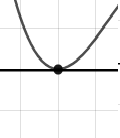
\includegraphics[width=0.3\textwidth]{../Figures/polyZeroBehaviorCA.png}
\end{center}\begin{enumerate}[label=\Alph*.]
\begin{multicols}{2}
\item 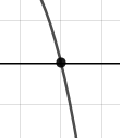
\includegraphics[width = 0.3\textwidth]{../Figures/polyZeroBehaviorAA.png}
\item 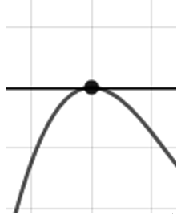
\includegraphics[width = 0.3\textwidth]{../Figures/polyZeroBehaviorBA.png}
\item 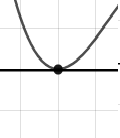
\includegraphics[width = 0.3\textwidth]{../Figures/polyZeroBehaviorCA.png}
\item 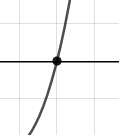
\includegraphics[width = 0.3\textwidth]{../Figures/polyZeroBehaviorDA.png}
\end{multicols}\item None of the above.\end{enumerate}
\textbf{General Comment:} You will need to sketch the entire graph, then zoom in on the zero the question asks about.
}
\litem{
Which of the following equations \textit{could} be of the graph presented below?

\begin{center}
    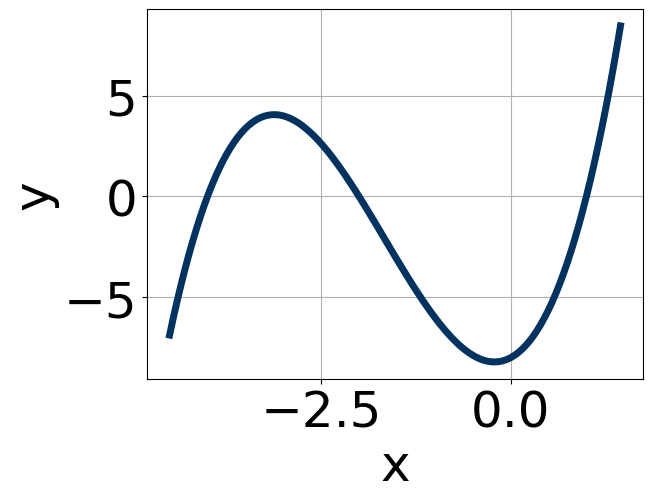
\includegraphics[width=0.5\textwidth]{../Figures/polyGraphToFunctionCopyA.png}
\end{center}




The solution is \( 12(x + 4)^{7} (x - 1)^{7} (x + 2)^{5} \), which is option E.\begin{enumerate}[label=\Alph*.]
\item \( 12(x + 4)^{10} (x - 1)^{11} (x + 2)^{5} \)

The factor $-4$ should have been an odd power.
\item \( 14(x + 4)^{10} (x - 1)^{6} (x + 2)^{11} \)

The factors $-4$ and $1$ have have been odd power.
\item \( -6(x + 4)^{6} (x - 1)^{5} (x + 2)^{9} \)

The factor $(x + 4)$ should have an odd power and the leading coefficient should be the opposite sign.
\item \( -9(x + 4)^{9} (x - 1)^{7} (x + 2)^{5} \)

This corresponds to the leading coefficient being the opposite value than it should be.
\item \( 12(x + 4)^{7} (x - 1)^{7} (x + 2)^{5} \)

* This is the correct option.
\end{enumerate}

\textbf{General Comment:} General Comments: Draw the x-axis to determine which zeros are touching (and so have even multiplicity) or cross (and have odd multiplicity).
}
\litem{
Describe the zero behavior of the zero $x = 7$ of the polynomial below.
\[ f(x) = -4(x + 2)^{5}(x - 2)^{3}(x + 7)^{7}(x - 7)^{6} \]

The solution is the graph below, which is option B.
\begin{center}
    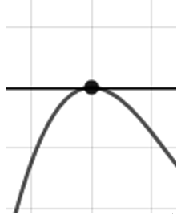
\includegraphics[width=0.3\textwidth]{../Figures/polyZeroBehaviorCopyBA.png}
\end{center}\begin{enumerate}[label=\Alph*.]
\begin{multicols}{2}
\item 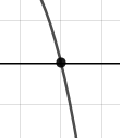
\includegraphics[width = 0.3\textwidth]{../Figures/polyZeroBehaviorCopyAA.png}
\item 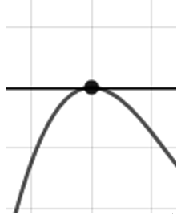
\includegraphics[width = 0.3\textwidth]{../Figures/polyZeroBehaviorCopyBA.png}
\item 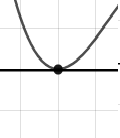
\includegraphics[width = 0.3\textwidth]{../Figures/polyZeroBehaviorCopyCA.png}
\item 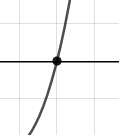
\includegraphics[width = 0.3\textwidth]{../Figures/polyZeroBehaviorCopyDA.png}
\end{multicols}\item None of the above.\end{enumerate}
\textbf{General Comment:} You will need to sketch the entire graph, then zoom in on the zero the question asks about.
}
\litem{
Which of the following equations \textit{could} be of the graph presented below?

\begin{center}
    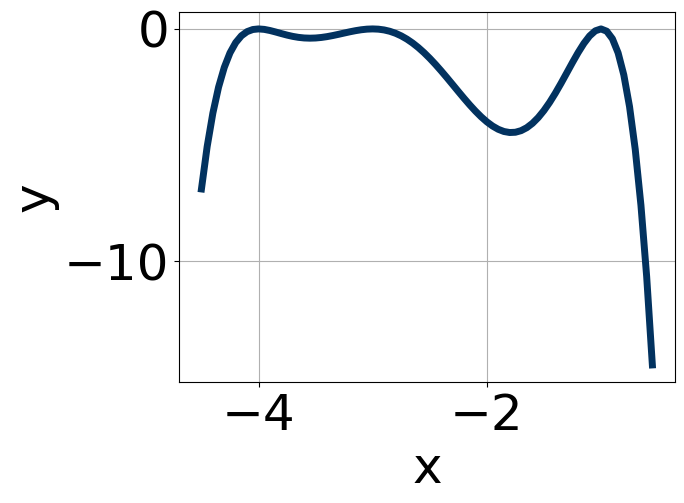
\includegraphics[width=0.5\textwidth]{../Figures/polyGraphToFunctionA.png}
\end{center}




The solution is \( -12(x + 3)^{10} (x + 4)^{6} (x + 1)^{4} \), which is option B.\begin{enumerate}[label=\Alph*.]
\item \( 10(x + 3)^{10} (x + 4)^{8} (x + 1)^{10} \)

This corresponds to the leading coefficient being the opposite value than it should be.
\item \( -12(x + 3)^{10} (x + 4)^{6} (x + 1)^{4} \)

* This is the correct option.
\item \( 7(x + 3)^{8} (x + 4)^{8} (x + 1)^{11} \)

The factor $(x + 1)$ should have an even power and the leading coefficient should be the opposite sign.
\item \( -6(x + 3)^{4} (x + 4)^{11} (x + 1)^{9} \)

The factors $(x + 4)$ and $(x + 1)$ should both have even powers.
\item \( -19(x + 3)^{6} (x + 4)^{8} (x + 1)^{7} \)

The factor $(x + 1)$ should have an even power.
\end{enumerate}

\textbf{General Comment:} General Comments: Draw the x-axis to determine which zeros are touching (and so have even multiplicity) or cross (and have odd multiplicity).
}
\litem{
Describe the end behavior of the polynomial below.
\[ f(x) = -8(x + 2)^{3}(x - 2)^{8}(x - 5)^{5}(x + 5)^{5} \]

The solution is the graph below, which is option A.
\begin{center}
    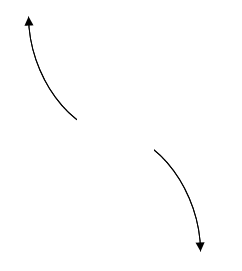
\includegraphics[width=0.3\textwidth]{../Figures/polyEndBehaviorCopyAA.png}
\end{center}\begin{enumerate}[label=\Alph*.]
\begin{multicols}{2}
\item 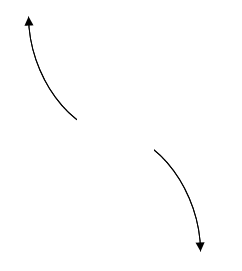
\includegraphics[width = 0.3\textwidth]{../Figures/polyEndBehaviorCopyAA.png}
\item 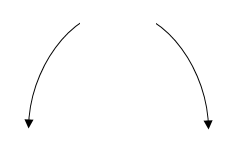
\includegraphics[width = 0.3\textwidth]{../Figures/polyEndBehaviorCopyBA.png}
\item 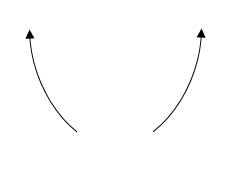
\includegraphics[width = 0.3\textwidth]{../Figures/polyEndBehaviorCopyCA.png}
\item 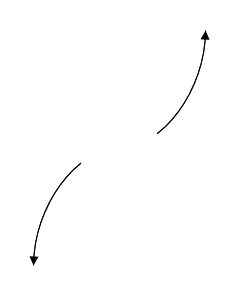
\includegraphics[width = 0.3\textwidth]{../Figures/polyEndBehaviorCopyDA.png}
\end{multicols}\item None of the above.\end{enumerate}
\textbf{General Comment:} Remember that end behavior is determined by the leading coefficient AND whether the \textbf{sum} of the multiplicities is positive or negative.
}
\litem{
Describe the end behavior of the polynomial below.
\[ f(x) = -5(x - 3)^{4}(x + 3)^{7}(x - 5)^{5}(x + 5)^{6} \]

The solution is the graph below, which is option B.
\begin{center}
    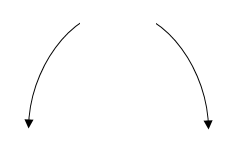
\includegraphics[width=0.3\textwidth]{../Figures/polyEndBehaviorBA.png}
\end{center}\begin{enumerate}[label=\Alph*.]
\begin{multicols}{2}
\item 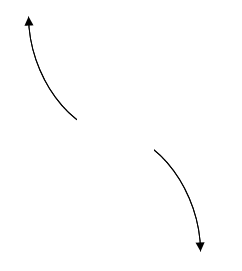
\includegraphics[width = 0.3\textwidth]{../Figures/polyEndBehaviorAA.png}
\item 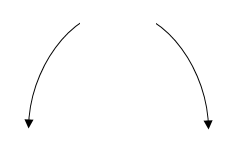
\includegraphics[width = 0.3\textwidth]{../Figures/polyEndBehaviorBA.png}
\item 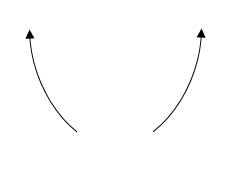
\includegraphics[width = 0.3\textwidth]{../Figures/polyEndBehaviorCA.png}
\item 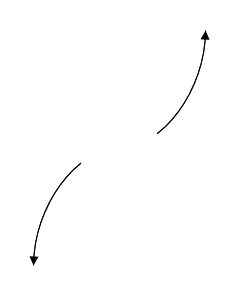
\includegraphics[width = 0.3\textwidth]{../Figures/polyEndBehaviorDA.png}
\end{multicols}\item None of the above.\end{enumerate}
\textbf{General Comment:} Remember that end behavior is determined by the leading coefficient AND whether the \textbf{sum} of the multiplicities is positive or negative.
}
\end{enumerate}

\end{document}